\documentclass[kulak]{kulakposter}
\usepackage[dutch]{babel}
\usepackage{graphicx}
\usepackage{amsmath}
\usepackage{hyperref}

\faculty{Teamopdracht 2023 -- 2024}
\title{Classificatie met een lineair SVM-model}
\author{Team \(\exists\)uler}
\institute{Vincent Van Schependom, Daan Vanhaverbeke, Jasper Benoit, Lasha Shergelashvili, Marie Taillieu, Zeineb Kharbach, Florian Degraeve, Younes Mebarki}
\photo{groepsfoto}

\newcommand{\norm}[1]{\left\| #1 \right\|}
\renewcommand{\boxed}[1]{\text{\fboxsep=.3em\fbox{#1}}}

\begin{document}

\maketitle

\begin{multicols}{2}
	\section*{Inleiding}
	\vspace{0.5cm}
	SVM of \textbf{Support Vector Machines} is een classificatietechniek. Indien elk punt in de dataset \(p\) verschillende \textit{features} heeft, zullen er \((p-1)\)-dimensionele objecten, genaamd hypervlakken (of \textit{hyperplanes}), berekend worden om de dataset in twee te groepen verdelen. Deze poster gaat over \textbf{lineaire} SVM, waarbij de datapunten worden gescheiden aan de hand van een \textbf{rechte}, dus er zijn twee features. (dit moet nog herwerkt worden)
	
%	 Deze poster gaat over \textbf{lineaire} SVM, waarbij de datapunten worden gescheiden aan de hand van een \textbf{rechte}. Een rechte is 1-dimensionaal, dus de inputs zien er als volgt uit: \[X = \left[ 
%	 \begin{array}{c}
%	 	x_1 \\
%	 	x_2
%	 \end{array} \right] \]
	\section{Classificatie}
	
	\vspace{1cm}
	\begin{multicols}{2}
		\textbf{Regressie:} \\
		
		Het vinden van een functie die zo goed mogelijk past op een dataset. Op basis van deze functie kunnen voorspellingen worden gemaakt voor nieuwe datapunten. \\
		
		De \textit{outputs} zijn \textbf{continue numerieke waarden} en kunnen heel veel waarden aannemen.
		
		\columnbreak
		\textbf{Classificatie:} \\
		
		Het onderverdelen van een dataset in meerdere, vooraf gedefinieerde, groepen. Op basis van de \textit{classifier} kan de groep van een nieuw datapunt voorspeld worden.\\
		
		De \textit{outputs} zijn \textbf{categorieën} en kunnen dus niet eender welke waarde aannemen.
		
	\end{multicols}
	
	\vspace{1.5cm}
	\textbf{Binaire} classificatie:
	\begin{itemize}
		\item Een punt behoort tot een van twee klassen
		\item \(y \in \{-1,1\}\)
		\item \(><\) \textit{multi-class} classificatie
	\end{itemize}
	\vfill \null
	
	\columnbreak
	\section{\textit{Maximum margin} hypervlakken}
	\begin{itemize}
		\item We stellen twee lineaire \textbf{hypervlakken} op met vergelijkingen:
			\[\vec{w} \cdot \vec{x} - b = 1 \quad \text{en} \quad \vec{w} \cdot \vec{x} - b = -1\]
			Omdat we met 2 features werken komt dit neer op:
			\[w_1x_1 + w_2x_2 - b = 1 \quad \text{en} \quad w_1x_1 + w_2x_2 - b = -1\]
	\end{itemize}
		\begin{itemize}
			\item \(\vec{w}\) is de \textbf{normaalvector} op de hypervlakken
			\item \(b\) is de \textit{\textbf{intercept}} van de rechte die de beslissingsrechte beschrijft
		\end{itemize}
	\photohere
	\centering
	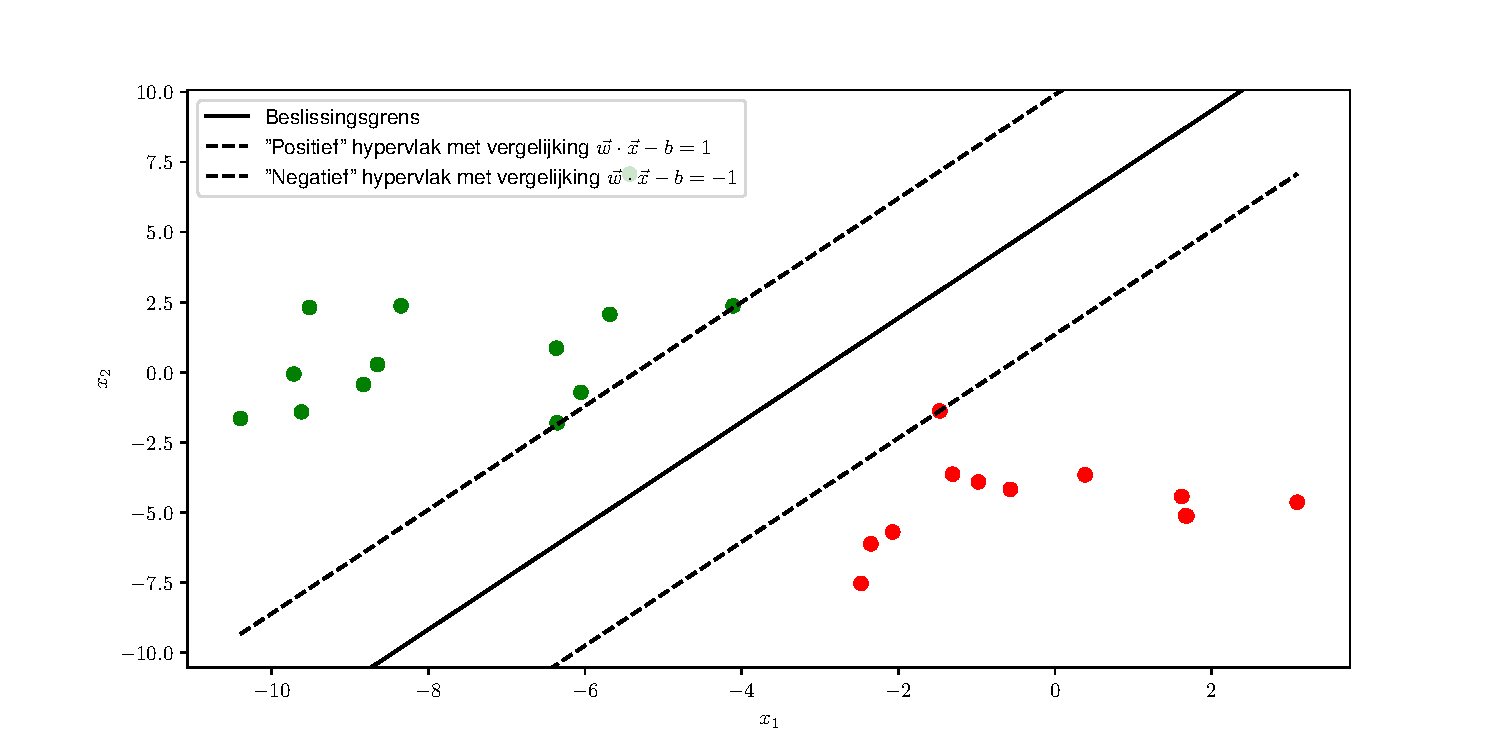
\includegraphics[width=.6\columnwidth]{hypervlakken}
	\begin{itemize}
		\item De \textbf{beslissingsgrens} ligt in het midden van beide hypervlakken
		\item Maximalisatie van de \textbf{marge} tussen de twee hypervlakken:
	\end{itemize}
	\centering
	\vspace{0.5cm}
	\(\frac{2}{\norm{\vec{w}}}\) maximaliseren \(\Rightarrow\) \(\norm{\vec{w}}\) minimaliseren
	
\end{multicols}
	
\begin{multicols}{2}
	
	\section{\textit{Hinge loss} \(l\)}
	
	De \textbf{\textit{hinge loss}} is een soort foutterm die als volgt gedefinieerd wordt:
	\[l=\max{(0,1-y_i(\vec{w}\cdot\vec{x}_i-b))}\]
	
	\vspace{0.5cm}
	
		\textbf{Goed geclassificeerde punten:}
		\begin{itemize}
			\item Aan de juiste kant van het positief/negatief hypervlak
			\item 	\(\left. \begin{array}{ll}
				\vec{w}\cdot \vec{x}_i-b\geq 1 & \text{als } y_i=1 \\
				\vec{w}\cdot \vec{x}_i-b\leq -1 & \text{als } y_i=-1
			\end{array} \right\} \Rightarrow y_i(\vec{w}\cdot \vec{x}_i-b)\geq 1 \Rightarrow \boxed{$l=0$} \)
		\end{itemize}
		\vspace{0.5cm}
		\textbf{Slecht geclassificeerde punten:}\\
		Twee opties:
		\begin{itemize}
			\item In de marge \(\Rightarrow\) \boxed{$0<l\leq 1$}
			\item Aan de foute kant van de beslissingsgrens \(\Rightarrow\) \boxed{$l > 1$}
		\end{itemize}
	
\section{Kostfunctie \(J\)}
\begin{multicols}{2}
	Optimaal model:
	\begin{itemize}
		\item Maximale marge \(\rightarrow\) minimale \(\norm{\vec{w}}\)
		\item Maximale accuraatheid \(\rightarrow\) minimale \(l\)
	\end{itemize}
	\columnbreak
	Kostfunctie \(J\) minimaliseren:
	\[\min_{w,b}J=\min_{w,b}\left(\frac{1}{n} \sum_{i=1}^n{\max{l_i}} + \lambda\cdot{||\vec{w}||}^2\right)\]
\end{multicols}

\columnbreak

\section{Regularisatieparameter \(\lambda\)}

De metaparameter wordt bij SVM de \textbf{regularisatieparameter} genoemd, aangeduid met \(\lambda\).

Deze \(\lambda\) heeft invloed op de minimalisatie van \(J\):

\begin{itemize}
\item Kleine \(\lambda\) \(\rightarrow\) zo veel mogelijk \textit{hinge losses} op 0 zetten \(\rightarrow\) \boxed{kleine marge} 
\item Grote \(\lambda\) \(\Rightarrow\) meer nadruk op het minimaliseren van de grootte van \(\norm{\vec{w}}\) \(\Rightarrow\) \boxed{grote marge}
\end{itemize}

\photohere
\centering
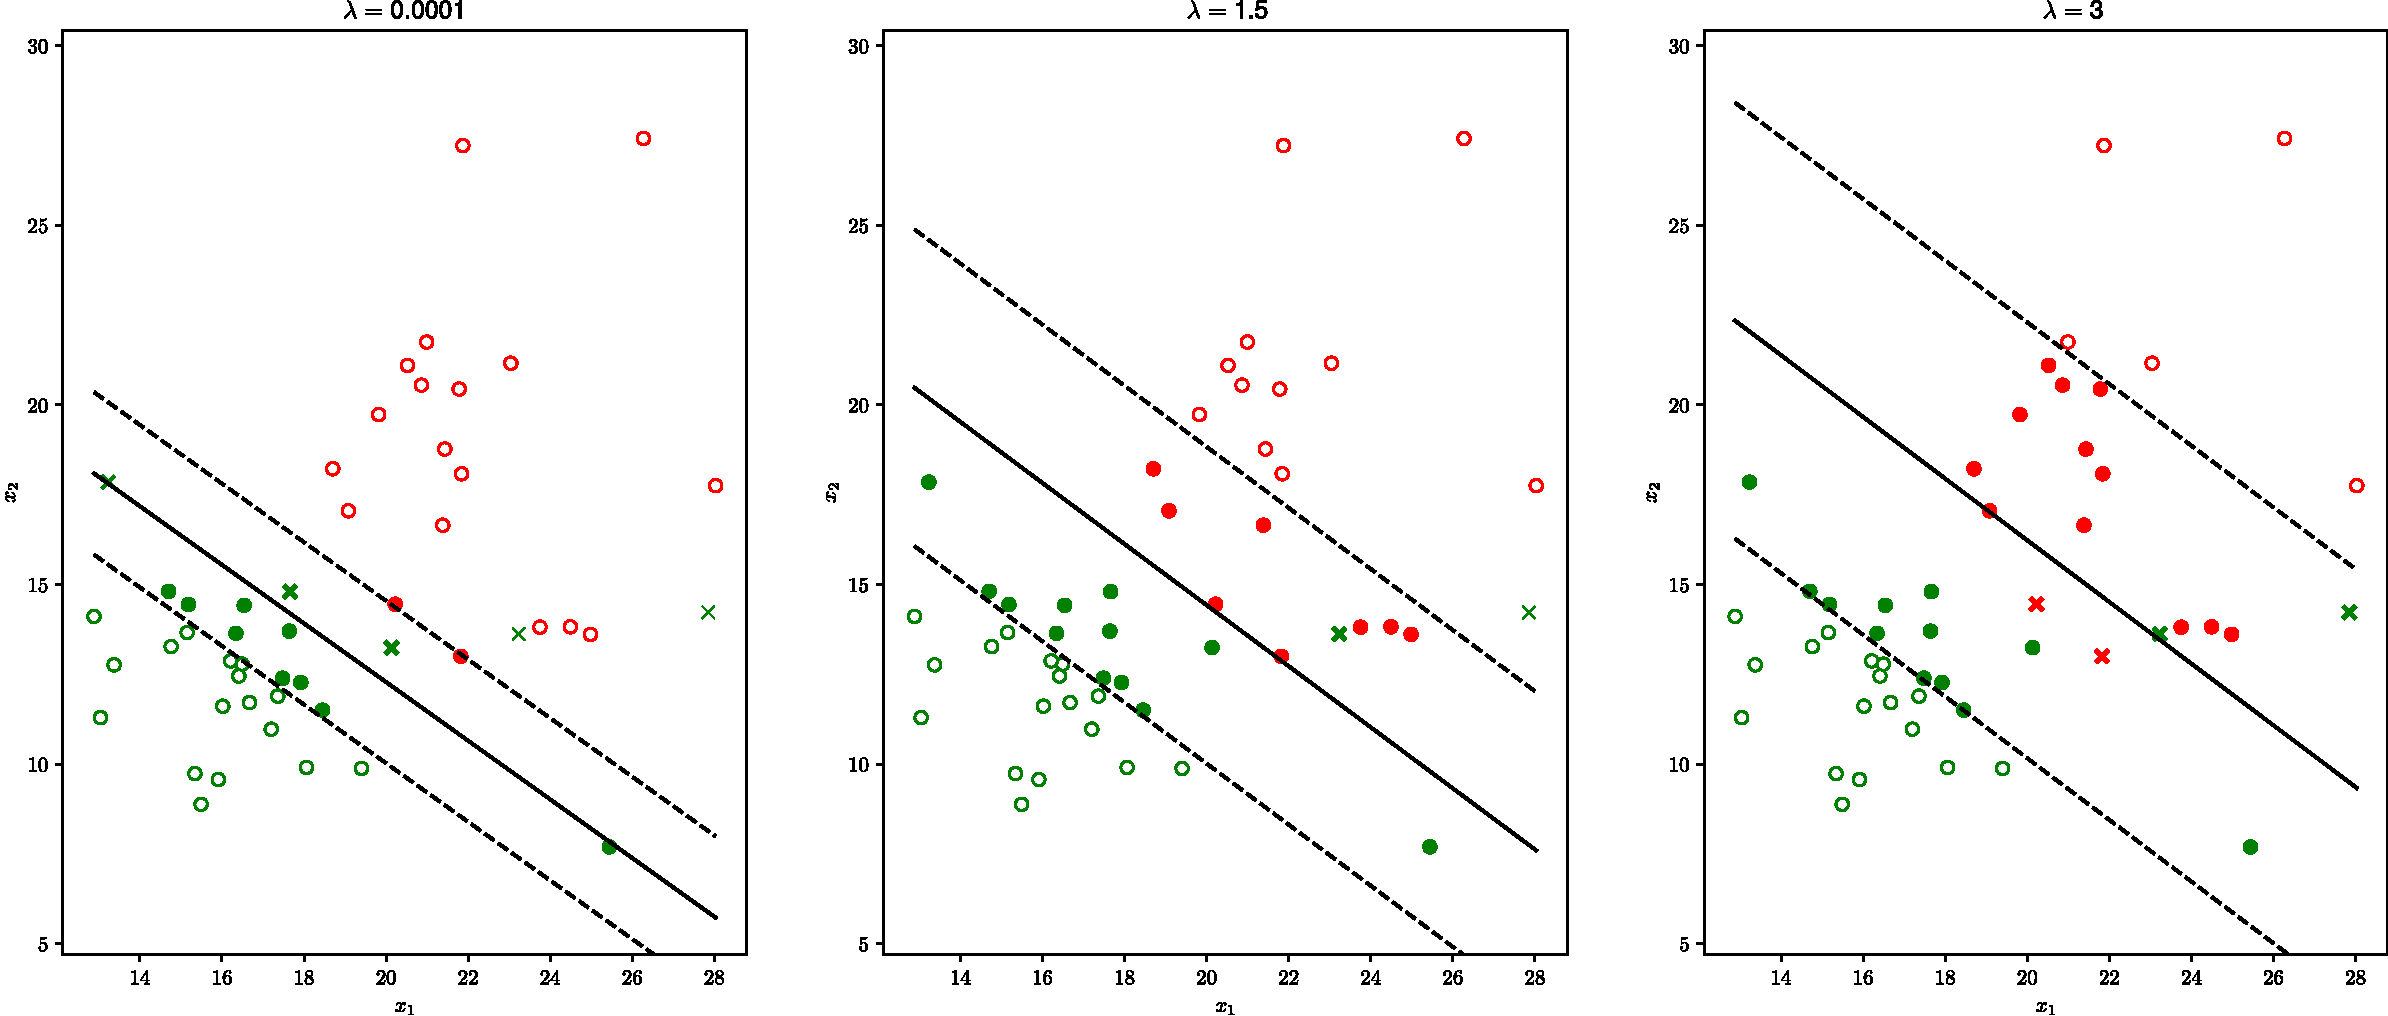
\includegraphics[width=.94\columnwidth]{regularisatieparameter}

\end{multicols}
\begin{multicols}{2}
\section{Voordelen van SVM}

\subsection{Hogere dimensies \& kleine datasets}

SVM werkt goed in hogere dimensies, met name wanneer het aantal \textit{features} groter is dan het aantal datapunten.

\subsection{Weinig last van \textit{overfitting}}

Dankzij het \textit{maximum margin} principe zijn Support Vector Machines niet gevoelig aan \textit{overfitting} en hebben \textit{outliers} niet veel invloed op het model.

\subsection{Geheugenefficiëntie}

Enkel de \textbf{\textit{support vectors}} - de dichtstbijzijnde punten tot de hypervlakken - spelen een rol in de berekening van het model.
	
	\columnbreak
	\section{Vergelijking met andere classificatietechnieken}
\end{multicols}


\section*{Besluit}
\begin{multicols}{2}\setlength{\columnseprule}{0pt}
Afsluitende tekst.
\end{multicols}

\nocite{mediumarticle}

\bibliography{referenties}
\bibliographystyle{unsrt}

\end{document}
